\subsection{Action categories}
\label{ssec:action_methods_actioncategories}

In this section, we will first define the action domain.
Here, the focus lies on actions involving hands and objects (and thus not gestures, \etc).
Reasoning about actions seemed for a long time of purely philosophical interest and a detailed review can be found in~\cite{aune1977reason}.
The same author states the major viewpoints~\cite{worgotter2013simple} on action ontologies as:~\cite[p. 195]{aune1988action}

\begin{quote}
``Perhaps the most controversial aspect of so called action theory is its subject matter.
This subject matter is generally said to be (or to concern) actions, but different philosophers conceive of actions in radically different ways. 
For some philosophers actions are abstract entities – states of affairs, propositions, sets, or even ordered pairs of some kind. 
For others, actions are distinctively concrete entities located in space and time. 
Another group of philosophers, among whom I include myself, have even denied that actions are required for a reasonable action theory, insisting that agents or actors will suffice as the theory's sole objects.''
\end{quote}

However, apart from the entity concept of an action, one needs to ask the question: ``What is an object?''
Originally, this subject was perceived as bottom-up and being object-driven.
This means different objects allow for different actions.
This is the so-called affordance principle~\cite{shaw2017perceiving}.

As stated in~\cite{worgotter2013simple} agency on the other hand suggests that the intended action lets the agent seek for appropriate objects.
This point of view leads away from the question ``What can you do with all the things in the world'', but rather points to the question of ``What can you do with your hands?'' and recent concepts suggest that objects and actions are intertwined~\cite{turchin1993cybernetic}.
In~\textcite{worgotter2013simple} it is shown that based on touching relations one can separate actions naturally.
This concept is introduced in the following sections in more detail.

Also stemming from this concept in~\cite{worgotter2013simple} an action ontology is derived, which assumes 26 atomic one-handed actions as shown in \tabref{tab:sec_definitionofactions_actiontable}.
Every sequence of actions, \eg ``make a sandwich'', can be broken down into a sequence of atomic actions:

\begin{table}[]
\resizebox{\textwidth}{!}{%
  \centering
  \begin{tabular}{cccll}
    \toprule
    Nr  & Type  & Goal  & Instantiation & Example\\
    \midrule
    1   & 1 & r     & Punch/hit         & with your hand an object\\
    2   & 1 & r     & Flick             & with your finger nail, quickly\\
    3   & 1 & r     & Poke              & with your finger tip, slowly\\
    4   & 1 & d     & Chop              & quickly, with the edge of your hand\\
    5   & 1 & r     & Turn = bore (rotate wrist x) & a hole with your finger or your hand\\
    6   & 1 & d     & Cut               & slowly, with the edge of your hand\\
    7   & 1 & d/r   & Scratch           & with your finger nail\\
    8   & 1 & d     & Scissor-cut/pinch & between your fingers\\
    9   & 1 & d/r   & Squash, squeeze   & inside your fist\\
    10  & 1 & d     & Draw              & with finger in sand\\
    11  & 1 & r     & Push/pull-without-grasp & regular push, hook-pull, adduct with finger\\
    12  & 1 & r     & Stir              & with finger\\
    13  & 1 & r     & Knead             & kneading dough, \etc\\
    14  & 1 & r     & Rub/massage       & with your hand someone else's body\\
    15  & 1 & r     & Lever (rotate wrist y)    & \eg break open a hole\\
    16  & 1 & d     & Scoop/ladle       & fill your hand with liquid\\
    \midrule
    17  & 2 & t     & Take Down or Pick apart   & one block from a laterally connected\\
        &   &       &                           & group or a pile by pick \& place\\
    18  & 2 & t     & Push down or push apart   & one block from a laterally connected\\
        &   &       &                           & group or a pile by pushing\\
    19  & 2 & b     & Rip off           & Rip a piece off an object\\
    20  & 2 & b     & Break off         & Break a piece off an object\\
    21  & 2 & b     & Uncover by pick \& place    & Pick off an object to uncover another\\
        &   &       &                           & object\\
    22  & 2 & b     & Uncover by pushing        & Push off an object to uncover another\\
        &   &       &                           & object\\
    \midrule
    23  & 3 & c     & Put on top or Put together    & two blocks on top of each other or side\\
        &   &       &                               & by side by pick \& place\\
    24  & 3 & c     & Push on top or push together  & two blocks on top of each other or side\\
        &   &       &                               & by side by pushing\\
    25  & 3 & h     & Put over          & Put one object above another one to\\
        &   &       &                   & cover it completely\\
    26  & 3 & h     & Push over         & Push one object above another one to\\
        &   &       &                   & cover it completely\\
    \bottomrule
  \end{tabular}
}
  \caption{List of atomic actions as taken from~\cite{worgotter2013simple}. 
      More actions are listed as ``Some (sic) dynamic versions of 17 -- 26''; for example, the action ``throw-in''.
      According to~\cite{worgotter2013simple} there are three different manipulation types (listed in the ``Type'' column): 1: Hand-only-actions; 2: Separation actions; 3: Release determined actions.
      Abbreviations in the ``Goal'' column are defined as follows: d: destroying; r: rearranging; c: constructing; t: taking-down; h: hiding; and b: breaking.}
  \label{tab:sec_definitionofactions_actiontable}
\end{table}

\begin{enumerate}
  \item \action{Pick \& Place} the bread from the table on the cutting board,
  \item \action{Cut} the bread,
  \item \action{Scoop} marmelade,
  \item \action{Put} marmelade \action{on top} of the bread.
\end{enumerate}

Each action is categorized into three types and each type into two goal categories:

\begin{enumerate}
  \item Hand-only actions:
    \begin{itemize}
      \item Rearrange (\eg hit, push, stir),
      \item Destroy (\eg cut, draw, scoop),
    \end{itemize}
  \item Separation actions:
    \begin{itemize}
      \item Take-down (\eg take-down, push apart)
      \item Break (\eg rip off, uncover by pick \& place),
    \end{itemize}
  \item Release determined actions:
    \begin{itemize}
      \item Construct (\eg put on top, push together),
      \item Hide (\eg. put over, push over),
    \end{itemize}
\end{enumerate}

where actions from each goal category share similar trajectories.
Next, one needs to define object roles.
These roles are determined by the changes that occur following an action in the relation of an object to other objects. 
An action involves at least two objects: a \emph{hand} and a \emph{main} object. 
The resulting object list (\emph{hand}, \emph{main}, \emph{primary}, \emph{secondary}, \etc) and their abstract roles are as followed (taken from~\textcite{reichaeinwoergoetter2018}):

\begin{itemize}
  \item \emph{Hand} (The object that performs the action): not touching anything at the beginning and the end of the action. It touch\-es at least one object during the manipulation.
  \item \emph{Main} (The object which is directly in contact with the hand): not touching the hand at the beginning and the end of action. It touches the hand at least once during the manipulation.
  \item \emph{Primary} (The object from which the \emph{main} object separates): initially touches the \emph{main} object. Changes its relation to not-touching during the action.
  \item \emph{Secondary} (The object to which the \emph{main} object joins): initially does not touch the \emph{main} object. Changes its relation to touching during the action.
  \item \emph{Load} (The object which is indirectly manipulated): does not touch the hand. This object touches/ untouches the \emph{main} and untouches/ touches the \emph{container} during the action .
  \item \emph{Container} (The object whose relation with \emph{load} changes and which is not the \emph{main} object): touches or untouches the \emph{load} object.
  \item \emph{Main support} (The object on which the \emph{main} object is located): touching the \emph{main} object at least once.
  \item \emph{Primary support} (The object on which the \emph{primary} object is located): touching the \emph{primary} object at least once.
  \item \emph{Secondary support} (The object on which the \emph{secondary} is located): touching the \emph{secondary} object at least once.
  \item \emph{Tool} (The object which is used by the hand to enhance the quality of some actions): touching the hand all the time.
\end{itemize}

When looking at object roles a different categorization of actions comes to mind: One can define action categories based upon the objects, which the hand interacts with.
These fall into three classes:

\begin{enumerate}
  \item Actions with \emph{main support}: In this category the \emph{main} object is always in touch with the \emph{main support}; an example is shown in \figref{fig:sec_definitionofactions_actionscategory_1}.
  \item Actions without \emph{main support}: In this category the \emph{main} object is lifted from the \emph{primary} object; an example is shown in \figref{fig:sec_definitionofactions_actionscategory_2}.
  \item Actions with \emph{load} and \emph{container}: In this category a \emph{container} with \emph{load}, \eg a glass filled with water, is used; an example is shown in \figref{fig:sec_definitionofactions_actionscategory_3}.
\end{enumerate}

A detailed list of actions is shown in \tabref{tab:sec_definitionofactions_ontologysummary}.
While the first categorization places its focus on the high level goal of the action, the second one is derived from the bottom-up point of view of an object's structural role.
In the following sections we will see that the structural role is also important for affordance and planning.

\begin{table}[]
  \begin{tabular}{p{3cm} p{6cm} p{3cm}}
    \toprule
    \multirow{2}{*}{Category}   & \multirow{2}{*}{Sub-Category} & Example\\
                                &                               & Actions\\
    \midrule
    \multirow{4}{3.0cm}{\vspace{1.5cm} \textcolor{white}{~~~~~~~~~~~~~~~~~} Actions with main support} & Actions with hand, main, and main support      & push, punch, flick\\ \cmidrule(l){2-3}
                & Actions with hand, main, main support, and primary                 & push apart, cut, chop\\ \cmidrule(l){2-3}
                & Actions with hand, main, main support, and secondary               & push together\\ \cmidrule(l){2-3}
                & Actions with hand, main, main support, primary, and secondary      & push from a to b\\
    \midrule
    \multirow{5}{3.0cm}{\vspace{1.5cm} \textcolor{white}{~~~~~~~~~~~~~~~~~} Actions without main support (These action have primary, secondary and their supports)}  & primary $\ne$ secondary and primary support $\ne$ secondary support  & pick and place, break off\\ \cmidrule(l){2-3}\
                & primary $\ne$ secondary and primary support $=$ secondary support & pick and place, break off\\ \cmidrule(l){2-3}
                & primary $\ne$ secondary and primary $=$ secondary support         & put on top\\ \cmidrule(l){2-3}
                & primary $\ne$ secondary and primary support $=$ secondary         & pick apart\\ \cmidrule(l){2-3}
                & primary $=$ secondary                                             & pick and place, break off \\
    \midrule
    \multirow{2}{3.0cm}{\vspace{-0.25cm} \textcolor{white}{~~~~~~~~~~~~~~~~~} Actions with load and~container} & The relation of load and main changes from N to T (loading)    & Pipetting\\ \cmidrule(l){2-3}
                & The relation of load and main changes from T to N  (unloading)    & Pour, Drop\\
    \bottomrule
  \end{tabular}
  \caption{Summary of ontology of actions. Actions are divided into three categories and further into sub-categories. There can be more than one action in each sub-category. Taken from~\textcite{reichaeinwoergoetter2018}.}
  \label{tab:sec_definitionofactions_ontologysummary}
\end{table}

\begin{figure}[]
  \begin{subfigure}[]{\textwidth}
    \centering
    % Define block styles
\tikzstyle{block} = [rectangle, fill=white, text width=1em, text centered, minimum height=0.5em, rounded corners=true]
\tikzstyle{blockBox} = [draw, rectangle, fill=white, minimum height=2.5cm, minimum width=4.5cm, text width=1em, text centered, rounded corners=true]

\tikzstyle{blockSupP} = [draw, rectangle, fill=red1!20, minimum height=0.6cm, minimum width=1.3cm, text width=1em, text centered, rounded corners=true]
\tikzstyle{blockSupM} = [draw, rectangle, fill=green1!20, minimum height=0.6cm, minimum width=1.3cm, text width=1em, text centered, rounded corners=true]
\tikzstyle{blockSupS} = [draw, rectangle, fill=blue1!20, minimum height=0.6cm, minimum width=1.3cm, text width=1em, text centered, rounded corners=true]
\tikzstyle{blockSup} = [draw, rectangle, fill=red1!20, minimum height=0.6cm, minimum width=3.5cm, text width=3.5cm, text centered, rounded corners=true]

\tikzstyle{blockCon} = [draw, rectangle, fill=white, minimum height=0.5cm, minimum width=1cm, text width=0.6cm, text centered, rounded corners=true]
\tikzstyle{blockP} = [draw, rectangle, fill=red1!40, minimum height=0.6cm, minimum width=0.6cm, text width=1em, text centered, rounded corners=true]
\tikzstyle{blockM} = [draw, rectangle, fill=green1!40, minimum height=0.6cm, minimum width=0.6cm, text width=1em, text centered, rounded corners=true]
\tikzstyle{blockS} = [draw, rectangle, fill=blue1!40, minimum height=0.6cm, minimum width=0.6cm, text width=1em, text centered, rounded corners=true]
\tikzstyle{blockL} = [draw, rectangle, fill=black!20, minimum height=0.6cm, minimum width=0.6cm, text width=1em, text centered, rounded corners=true]
\tikzstyle{arrow} = [draw, -latex]

\definecolor{red1}{RGB}{160,0,0}
\definecolor{green1}{RGB}{0,160,0}
\definecolor{blue1}{RGB}{0,0,160}

\pgfdeclareimage[width=0.6cm]{hand}{./figures/sec/robothand.jpg}

	      
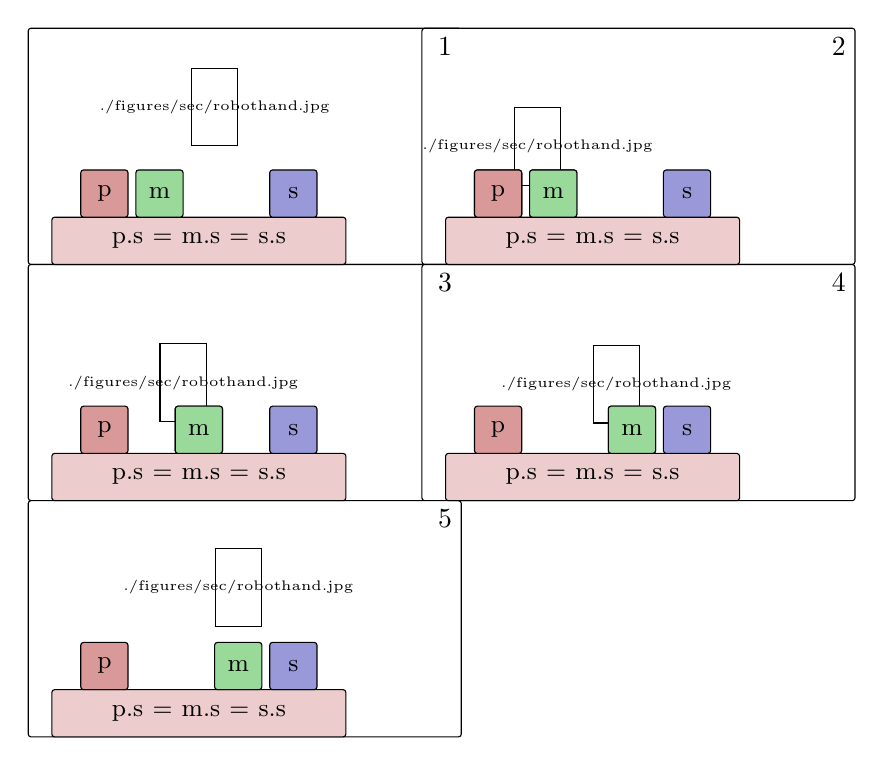
\begin{tikzpicture}[node distance=6em, auto]
	%%%%%%%%%%%%%%%%%%%%%%%%%%%%%%%%%%%%%%%%%%%%%%%%%%%%%%%%%%%%%%%%%%%%%%%%%%%%%%%%%%%%%%%%%%%%%%%%%%%%%%
	% First line
	\node [blockBox] (p11) {};
	\node [blockBox, right of=p11, node distance=5cm] (p12) {};
	\node [blockBox, below of=p11, node distance=3.0cm] (p13) {};
	\node [blockBox, right of=p13, node distance=5cm] (p14) {};
	\node [blockBox, below of=p13, node distance=3.0cm] (p15) {};

	% Panel number
	\node[below left] at (p11.north east) {1};
	\node[below left] at (p12.north east) {2};
	\node[below left] at (p13.north east) {3};
	\node[below left] at (p14.north east) {4};
	\node[below left] at (p15.north east) {5};

	% Panel 11
	\node [above right, xshift=0.3cm, blockSup, minimum width=3cm] at (p11.south west) (p11_Sup) {\small{p.s~=~m.s~=~s.s}};

	\node [above of=p11_Sup, blockP, node distance=0.6cm, xshift=-1.2cm] (p11_p) {\small{p}};
	\node [above of=p11_Sup, blockM, node distance=0.6cm, xshift=-0.5cm] (p11_m) {\small{m}};
	\node [above of=p11_Sup, blockS, node distance=0.6cm, xshift= 1.2cm] (p11_s) {\small{s}};

	\node [above of=p11_p, node distance=1.1cm, xshift=1.4cm] (p11_h) {\pgfuseimage{hand}};

	% Panel 12
	\node [above right, xshift=0.3cm, blockSup, minimum width=3cm] at (p12.south west) (p12_Sup) {\small{p.s~=~m.s~=~s.s}};

	\node [above of=p12_Sup, blockP, node distance=0.6cm, xshift=-1.2cm] (p12_p) {\small{p}};
	\node [above of=p12_Sup, blockM, node distance=0.6cm, xshift=-0.5cm] (p12_m) {\small{m}};
	\node [above of=p12_Sup, blockS, node distance=0.6cm, xshift= 1.2cm] (p12_s) {\small{s}};

	\node [above of=p12_m, node distance=0.6cm, xshift=-0.2cm] (p12_h) {\pgfuseimage{hand}};
	\node [above of=p12_Sup, blockP, node distance=0.6cm, xshift=-1.2cm] (p12_p) {\small{p}};
	\node [above of=p12_Sup, blockM, node distance=0.6cm, xshift=-0.5cm] (p12_m) {\small{m}};

	% Panel 13
	\node [above right, xshift=0.3cm, blockSup, minimum width=3cm] at (p13.south west) (p13_Sup) {\small{p.s~=~m.s~=~s.s}};

	\node [above of=p13_Sup, blockP, node distance=0.6cm, xshift=-1.2cm] (p13_p) {\small{p}};
	\node [above of=p13_Sup, blockM, node distance=0.6cm, xshift= 0.0cm] (p13_m) {\small{m}};
	\node [above of=p13_Sup, blockS, node distance=0.6cm, xshift= 1.2cm] (p13_s) {\small{s}};

	\node [above of=p13_m, node distance=0.6cm, xshift=-0.2cm] (p13_h) {\pgfuseimage{hand}};
	\node [above of=p13_Sup, blockM, node distance=0.6cm, xshift= 0.0cm] (p13_m) {\small{m}};

	% Panel 14
	\node [above right, xshift=0.3cm, blockSup, minimum width=3cm] at (p14.south west) (p14_Sup) {\small{p.s~=~m.s~=~s.s}};

	\node [above of=p14_Sup, blockP, node distance=0.6cm, xshift=-1.2cm] (p14_p) {\small{p}};
	\node [above of=p14_Sup, blockM, node distance=0.6cm, xshift= 0.5cm] (p14_m) {\small{m}};
	\node [above of=p14_Sup, blockS, node distance=0.6cm, xshift= 1.2cm] (p14_s) {\small{s}};

	\node [above of=p14_m, node distance = 0.58cm, xshift=-0.2cm] (p14_h) {\pgfuseimage{hand}};
	\node [above of=p14_Sup, blockM, node distance=0.6cm, xshift= 0.5cm] (p14_m) {\small{m}};

	% Panel 15
	\node [above right, xshift=0.3cm, blockSup, minimum width=3cm] at (p15.south west) (p15_Sup) {\small{p.s~=~m.s~=~s.s}};

	\node [above of=p15_Sup, blockP, node distance=0.6cm, xshift=-1.2cm] (p15_p) {\small{p}};
	\node [above of=p15_Sup, blockM, node distance=0.6cm, xshift= 0.5cm] (p15_m) {\small{m}};
	\node [above of=p15_Sup, blockS, node distance=0.6cm, xshift= 1.2cm] (p15_s) {\small{s}};

	\node [above of=p15_m, node distance = 1cm] (p15_h) {\pgfuseimage{hand}};
\end{tikzpicture}

    \caption{Example action with \emph{main support}: \action{Pushing}.}
    \label{fig:sec_definitionofactions_actionscategory_1}
  \end{subfigure}
  \begin{subfigure}[]{\textwidth}
    \centering
    % Define block styles
\tikzstyle{block} = [rectangle, fill=white, text width=1em, text centered, minimum height=0.5em, rounded corners=true]
\tikzstyle{blockBox} = [draw, rectangle, fill=white, minimum height=2.5cm, minimum width=4.5cm, text width=1em, text centered, rounded corners=true]

\tikzstyle{blockSupP} = [draw, rectangle, fill=red1!20, minimum height=0.6cm, minimum width=1.3cm, text width=1em, text centered, rounded corners=true]
\tikzstyle{blockSupM} = [draw, rectangle, fill=green1!20, minimum height=0.6cm, minimum width=1.3cm, text width=1em, text centered, rounded corners=true]
\tikzstyle{blockSupS} = [draw, rectangle, fill=blue1!20, minimum height=0.6cm, minimum width=1.3cm, text width=1em, text centered, rounded corners=true]
\tikzstyle{blockSup} = [draw, rectangle, fill=red1!20, minimum height=0.6cm, minimum width=3.5cm, text width=3.5cm, text centered, rounded corners=true]

\tikzstyle{blockCon} = [draw, rectangle, fill=white, minimum height=0.6cm, minimum width=1cm, text width=0.6cm, text centered, rounded corners=true]
\tikzstyle{blockP} = [draw, rectangle, fill=red1!40, minimum height=0.6cm, minimum width=0.6cm, text width=1em, text centered, rounded corners=true]
\tikzstyle{blockM} = [draw, rectangle, fill=green1!40, minimum height=0.6cm, minimum width=0.6cm, text width=1em, text centered, rounded corners=true]
\tikzstyle{blockS} = [draw, rectangle, fill=blue1!40, minimum height=0.6cm, minimum width=0.6cm, text width=1em, text centered, rounded corners=true]
\tikzstyle{blockL} = [draw, rectangle, fill=black!20, minimum height=0.6cm, minimum width=0.6cm, text width=1em, text centered, rounded corners=true]
\tikzstyle{arrow} = [draw, -latex]

\definecolor{red1}{RGB}{160,0,0}
\definecolor{green1}{RGB}{0,160,0}
\definecolor{blue1}{RGB}{0,0,160}

\pgfdeclareimage[width=0.6cm]{hand}{./figures/sec/robothand.jpg}

	      
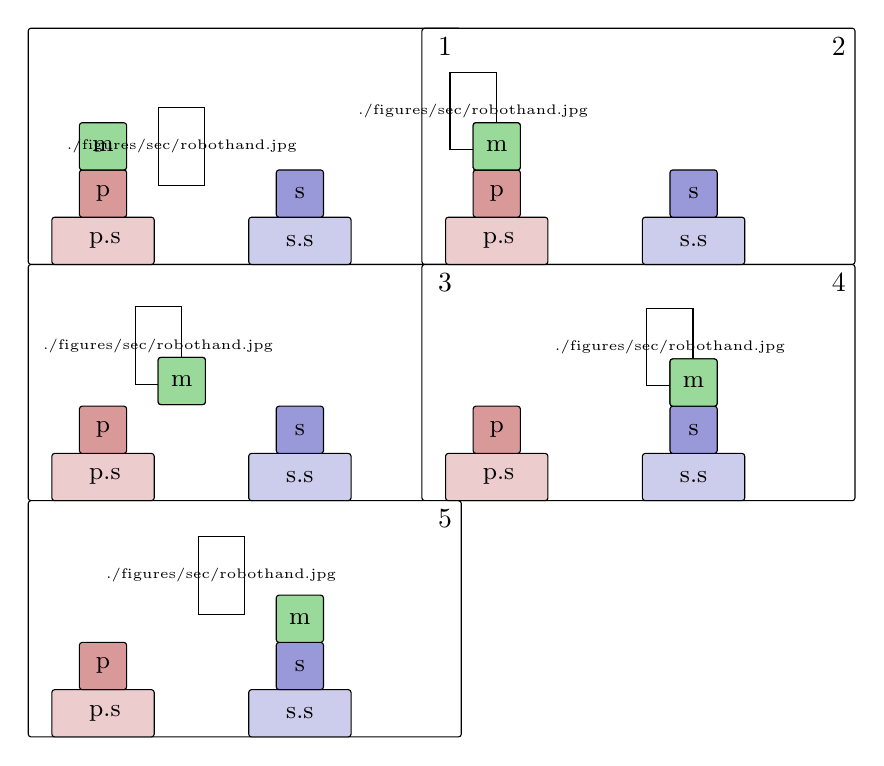
\begin{tikzpicture}[node distance=6em, auto]
	%%%%%%%%%%%%%%%%%%%%%%%%%%%%%%%%%%%%%%%%%%%%%%%%%%%%%%%%%%%%%%%%%%%%%%%%%%%%%%%%%%%%%%%%%%%%%%%%%%%%%%
	% second line
	\node [blockBox] (p21) {};
	\node [blockBox, right of=p21, node distance=5cm] (p22) {};
	\node [blockBox, below of=p21, node distance=3cm] (p23) {};
	\node [blockBox, right of=p23, node distance=5cm] (p24) {};
	\node [blockBox, below of=p23, node distance=3cm] (p25) {};

	% panel number
	\node[below left] at (p21.north east) {1};
	\node[below left] at (p22.north east) {2};
	\node[below left] at (p23.north east) {3};
	\node[below left] at (p24.north east) {4};
	\node[below left] at (p25.north east) {5};

	% Panel 21

	\node [above right, xshift=0.3cm, blockSupP] at (p21.south west) (p21_ps) {\small{p.s}};
	\node [right of=p21_ps, blockSupS, node distance=2.5cm] (p21_ss) {\small{s.s}};

	\node [above of=p21_ps, blockP, node distance=0.6cm] (p21_p) {\small{p}};
	\node [above of=p21_p, blockM, node distance=0.6cm] (p21_m) {\small{m}};
	\node [above of=p21_ss, blockS, node distance=0.6cm] (p21_s) {\small{s}};

	\node [above of=p21_m, node distance = 0.0cm, xshift=1cm] (p21_h) {\pgfuseimage{hand}};

	% Panel 22
	\node [above right, xshift=0.3cm, blockSupP] at (p22.south west) (p22_ps) {\small{p.s}};
	\node [right of=p22_ps, blockSupS, node distance=2.5cm] (p22_ss) {\small{s.s}};

	\node [above of=p22_ps, blockP, node distance=0.6cm] (p22_p) {\small{p}};
	\node [above of=p22_p, blockM, node distance=0.6cm] (p22_m) {\small{m}};
	\node [above of=p22_ss, blockS, node distance=0.6cm] (p22_s) {\small{s}};

	\node [above of=p22_m, node distance = 0.45cm, xshift=-0.3cm] (p22_h) {\pgfuseimage{hand}};
	\node [above of=p22_p, blockM, node distance=0.6cm] (p22_m) {\small{m}};

	% Panel 23
	\node [above right, xshift=0.3cm, blockSupP] at (p23.south west) (p23_ps) {\small{p.s}};
	\node [right of=p23_ps, blockSupS, node distance=2.5cm] (p23_ss) {\small{s.s}};

	\node [above of=p23_ps, blockP, node distance=0.6cm] (p23_p) {\small{p}};
	\node [above of=p23_p, blockM, node distance=0.62cm, xshift=1cm] (p23_m) {\small{m}};
	\node [above of=p23_ss, blockS, node distance=0.6cm] (p23_s) {\small{s}};

	\node [above of=p23_m, node distance = 0.45cm, xshift=-0.3cm] (p23_h) {\pgfuseimage{hand}};
	\node [above of=p23_p, blockM, node distance=0.62cm, xshift=1cm] (p23_m) {\small{m}};

	% Panel 24
	\node [above right, xshift=0.3cm, blockSupP] at (p24.south west) (p24_ps) {\small{p.s}};
	\node [right of=p24_ps, blockSupS, node distance=2.5cm] (p24_ss) {\small{s.s}};

	\node [above of=p24_ps, blockP, node distance=0.6cm] (p24_p) {\small{p}};
	\node [above of=p24_ss, blockS, node distance=0.6cm] (p24_s) {\small{s}};
	\node [above of=p24_s, blockM, node distance=0.6cm] (p24_m) {\small{m}};

	\node [above of=p24_m, node distance = 0.45cm, xshift=-0.3cm] (p24_h) {\pgfuseimage{hand}};
	\node [above of=p24_s, blockM, node distance=0.6cm] (p24_m) {\small{m}};

	% Panel 25
	\node [above right, xshift=0.3cm, blockSupP] at (p25.south west) (p25_ps) {\small{p.s}};
	\node [right of=p25_ps, blockSupS, node distance=2.5cm] (p25_ss) {\small{s.s}};

	\node [above of=p25_ps, blockP, node distance=0.6cm] (p25_p) {\small{p}};
	\node [above of=p25_ss, blockS, node distance=0.6cm] (p25_s) {\small{s}};
	\node [above of=p25_s, blockM, node distance=0.6cm] (p25_m) {\small{m}};

	\node [above of=p25_m, node distance = 0.55cm, xshift=-1.0cm] (p25_h) {\pgfuseimage{hand}};
\end{tikzpicture}

    \caption{Example action without \emph{main support}: \action{Pick and place}.}
    \label{fig:sec_definitionofactions_actionscategory_2}
  \end{subfigure}
\end{figure}
\begin{figure}[]\ContinuedFloat
  \begin{subfigure}[]{\textwidth}
    \centering
    % Define block styles
\tikzstyle{block} = [rectangle, fill=white, text width=1em, text centered, minimum height=0.5em, rounded corners=true]
\tikzstyle{blockBox} = [draw, rectangle, fill=white, minimum height=3cm, minimum width=5.5cm, text width=1em, text centered, rounded corners=true]

\tikzstyle{blockSupP} = [draw, rectangle, fill=red1!20, minimum height=0.6cm, minimum width=1.3cm, text width=1em, text centered, rounded corners=true]
\tikzstyle{blockSupM} = [draw, rectangle, fill=green1!20, minimum height=0.6cm, minimum width=1.3cm, text width=1em, text centered, rounded corners=true]
\tikzstyle{blockSupS} = [draw, rectangle, fill=blue1!20, minimum height=0.6cm, minimum width=1.3cm, text width=1em, text centered, rounded corners=true]
\tikzstyle{blockSup} = [draw, rectangle, fill=red1!20, minimum height=0.6cm, minimum width=3.5cm, text width=3.5cm, text centered, rounded corners=true]

\tikzstyle{blockCon} = [draw, rectangle, fill=white, minimum height=0.6cm, minimum width=1.3cm, text width=1.2cm, text centered, rounded corners=true]
\tikzstyle{blockP} = [draw, rectangle, fill=red1!40, minimum height=0.6cm, minimum width=0.6cm, text width=1em, text centered, rounded corners=true]
\tikzstyle{blockM} = [draw, rectangle, fill=green1!40, minimum height=0.6cm, minimum width=0.6cm, text width=1em, text centered, rounded corners=true]
\tikzstyle{blockS} = [draw, rectangle, fill=blue1!40, minimum height=0.6cm, minimum width=0.6cm, text width=1em, text centered, rounded corners=true]
\tikzstyle{blockL} = [draw, rectangle, fill=black!20, minimum height=0.6cm, minimum width=0.6cm, text width=1em, text centered, rounded corners=true]
\tikzstyle{arrow} = [draw, -latex]

\definecolor{red1}{RGB}{160,0,0}
\definecolor{green1}{RGB}{0,160,0}
\definecolor{blue1}{RGB}{0,0,160}

\pgfdeclareimage[width=0.6cm]{hand}{./figures/sec/robothand.jpg}

	      
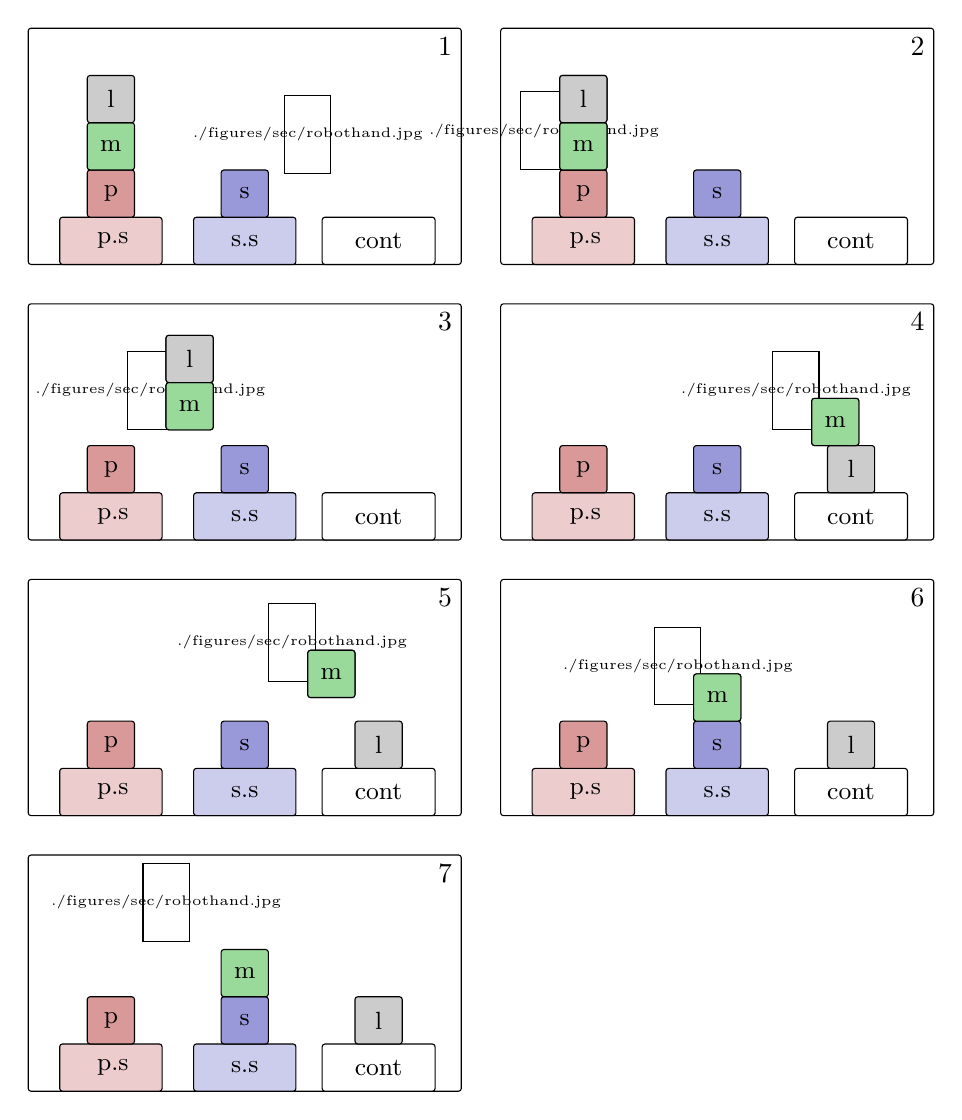
\begin{tikzpicture}[node distance=6em, auto]
	%%%%%%%%%%%%%%%%%%%%%%%%%%%%%%%%%%%%%%%%%%%%%%%%%%%%%%%%%%%%%%%%%%%%%%%%%%%%%%%%%%%%%%%%%%%%%%%%%%%%%%
	% third line
	\node [blockBox] (p31) {};
	\node [blockBox, right of=p31, node distance=6cm] (p32) {};
	\node [blockBox, below of=p31, node distance=3.5cm] (p33) {};
	\node [blockBox, right of=p33, node distance=6cm] (p34) {};
	\node [blockBox, below of=p33, node distance=3.5cm] (p35) {};

	\node [blockBox, right of=p35, node distance=6cm] (p36) {};
	\node [blockBox, below of=p35, node distance=3.5cm] (p37) {};

	% panel number
	\node[below left] at (p31.north east) {1};
	\node[below left] at (p32.north east) {2};
	\node[below left] at (p33.north east) {3};
	\node[below left] at (p34.north east) {4};
	\node[below left] at (p35.north east) {5};
	\node[below left] at (p36.north east) {6};
	\node[below left] at (p37.north east) {7};

	% Panel 31
	\node [above right, xshift=0.4cm, blockSupP] at (p31.south west) (p31_ps) {\small{p.s}};
	\node [right of=p31_ps, blockSupS, node distance=1.7cm] (p31_ss) {\small{s.s}};
	\node [right of=p31_ss, blockCon, node distance=1.7cm] (p31_con) {\small{cont}};

	\node [above of=p31_ps, blockP, node distance=0.6cm] (p31_p) {\small{p}};
	\node [above of=p31_p, blockM, node distance=0.6cm] (p31_m) {\small{m}};
	\node [above of=p31_m, blockL, node distance=0.6cm] (p31_l) {\small{l}};
	\node [above of=p31_ss, blockS, node distance=0.6cm] (p31_s) {\small{s}};

	\node [above of=p31_m, node distance = 0.15cm, xshift=2.5cm] (p31_h) {\pgfuseimage{hand}};

	% Panel 32
	\node [above right, xshift=0.4cm, blockSupP] at (p32.south west) (p32_ps) {\small{p.s}};
	\node [right of=p32_ps, blockSupS, node distance=1.7cm] (p32_ss) {\small{s.s}};
	\node [right of=p32_ss, blockCon, node distance=1.7cm] (p32_con) {\small{cont}};

	\node [above of=p32_ps, blockP, node distance=0.6cm] (p32_p) {\small{p}};
	\node [above of=p32_p, blockM, node distance=0.6cm] (p32_m) {\small{m}};
	\node [above of=p32_m, blockL, node distance=0.6cm] (p32_l) {\small{l}};
	\node [above of=p32_ss, blockS, node distance=0.6cm] (p32_s) {\small{s}};

	\node [above of=p32_m, node distance = 0.2cm, xshift=-0.5cm] (p32_h) {\pgfuseimage{hand}};
	\node [above of=p32_p, blockM, node distance=0.6cm] (p32_m) {\small{m}};
	\node [above of=p32_m, blockL, node distance=0.6cm] (p32_l) {\small{l}};

	% Panel 33
	\node [above right, xshift=0.4cm, blockSupP] at (p33.south west) (p33_ps) {\small{p.s}};
	\node [right of=p33_ps, blockSupS, node distance=1.7cm] (p33_ss) {\small{s.s}};
	\node [right of=p33_ss, blockCon, node distance=1.7cm] (p33_con) {\small{cont}};

	\node [above of=p33_ps, blockP, node distance=0.6cm] (p33_p) {\small{p}};
	\node [above of=p33_p, blockM, node distance=0.8cm, xshift=1cm] (p33_m) {\small{m}};
	\node [above of=p33_m, blockL, node distance=0.6cm] (p33_l) {\small{l}};
	\node [above of=p33_ss, blockS, node distance=0.6cm] (p33_s) {\small{s}};

	\node [above of=p33_m, node distance = 0.2cm, xshift=-0.5cm] (p33_h) {\pgfuseimage{hand}};
	\node [above of=p33_p, blockM, node distance=0.8cm, xshift=1cm] (p33_m) {\small{m}};
	\node [above of=p33_m, blockL, node distance=0.6cm] (p33_l) {\small{l}};

	% Panel 34
	\node [above right, xshift=0.4cm, blockSupP] at (p34.south west) (p34_ps) {\small{p.s}};
	\node [right of=p34_ps, blockSupS, node distance=1.7cm] (p34_ss) {\small{s.s}};
	\node [right of=p34_ss, blockCon, node distance=1.7cm] (p34_con) {\small{cont}};

	\node [above of=p34_ps, blockP, node distance=0.6cm] (p34_p) {\small{p}};
	\node [above of=p34_con, blockL, node distance=0.6cm] (p34_l) {\small{l}};
	\node [above of=p34_l, blockM, node distance=0.6cm, xshift=-0.2cm] (p34_m) {\small{m}};
	\node [above of=p34_ss, blockS, node distance=0.6cm] (p34_s) {\small{s}};

	\node [above of=p34_m, node distance=0.4cm, xshift=-0.5cm] (p34_h) {\pgfuseimage{hand}};
	\node [above of=p34_l, blockM, node distance=0.6cm, xshift=-0.2cm] (p34_m) {\small{m}};

	% Panel 35
	\node [above right, xshift=0.4cm, blockSupP] at (p35.south west) (p35_ps) {\small{p.s}};
	\node [right of=p35_ps, blockSupS, node distance=1.7cm] (p35_ss) {\small{s.s}};
	\node [right of=p35_ss, blockCon, node distance=1.7cm] (p35_con) {\small{cont}};

	\node [above of=p35_ps, blockP, node distance=0.6cm] (p35_p) {\small{p}};
	\node [above of=p35_con, blockL, node distance=0.6cm] (p35_l) {\small{l}};
	\node [above of=p35_l, blockM, node distance=0.9cm, xshift=-0.6cm] (p35_m) {\small{m}};
	\node [above of=p35_ss, blockS, node distance=0.6cm] (p35_s) {\small{s}};

	\node [above of=p35_m, node distance = 0.4cm, xshift=-0.5cm] (p35_h) {\pgfuseimage{hand}};
	\node [above of=p35_l, blockM, node distance=0.9cm, xshift=-0.6cm] (p35_m) {\small{m}};

	% Panel 36
	\node [above right, xshift=0.4cm, blockSupP] at (p36.south west) (p36_ps) {\small{p.s}};
	\node [right of=p36_ps, blockSupS, node distance=1.7cm] (p36_ss) {\small{s.s}};
	\node [right of=p36_ss, blockCon, node distance=1.7cm] (p36_con) {\small{cont}};

	\node [above of=p36_ps, blockP, node distance=0.6cm] (p36_p) {\small{p}};
	\node [above of=p36_con, blockL, node distance=0.6cm] (p36_l) {\small{l}};
	\node [above of=p36_ss, blockS, node distance=0.6cm] (p36_s) {\small{s}};
	\node [above of=p36_s, blockM, node distance=0.6cm] (p36_m) {\small{m}};

	\node [above of=p36_m, node distance = 0.4cm, xshift=-0.5cm] (p36_h) {\pgfuseimage{hand}};
	\node [above of=p36_s, blockM, node distance=0.6cm] (p36_m) {\small{m}};

	% Panel 37
	\node [above right, xshift=0.4cm, blockSupP] at (p37.south west) (p37_ps) {\small{p.s}};
	\node [right of=p37_ps, blockSupS, node distance=1.7cm] (p37_ss) {\small{s.s}};
	\node [right of=p37_ss, blockCon, node distance=1.7cm] (p37_con) {\small{cont}};

	\node [above of=p37_ps, blockP, node distance=0.6cm] (p37_p) {\small{p}};
	\node [above of=p37_con, blockL, node distance=0.6cm] (p37_l) {\small{l}};
	\node [above of=p37_ss, blockS, node distance=0.6cm] (p37_s) {\small{s}};
	\node [above of=p37_s, blockM, node distance=0.6cm] (p37_m) {\small{m}};

	\node [above of=p37_m, node distance = 0.9cm, xshift=-1cm] (p37_h) {\pgfuseimage{hand}};
\end{tikzpicture}

    \caption{Example action with \emph{load} and \emph{container}: \action{Unloading}. The \emph{main} object m could be, for example, a glass and the \emph{load} l could be water. The water is unloaded into a flower pot.}
    \label{fig:sec_definitionofactions_actionscategory_3}
  \end{subfigure}
  \caption{Schematic example actions in the ontology are shown for the three categories.
  From each category only one action is shown.
  The objects are marked using the following convention:
  h~=~hand, m~=~main m.s~=~main support, p~=~primary, p.s~=~primary support, s~=~secondary, s.s~=~secondary support, l~=~load, and cont~=~container (taken from~\textcite{reichaeinwoergoetter2018}).}
  \label{fig:sec_definitionofactions_ontologyactions}
\end{figure}
